\documentclass[a4paper, 10pt, twoside]{article}

\usepackage[top=1in, bottom=1in, left=1in, right=1in]{geometry}
\usepackage[utf8]{inputenc}
\usepackage[spanish, es-ucroman, es-noquoting]{babel}
\usepackage{setspace}
\usepackage{fancyhdr}
\usepackage{lastpage}
\usepackage{amsmath}
\usepackage{amsfonts}
\usepackage{amsthm}
\usepackage{verbatim}
\usepackage{graphicx}
\usepackage{float}
\usepackage[noend]{algpseudocode}
\usepackage{enumitem} % Provee macro \setlist
\usepackage[toc, page]{appendix}


%%%%%%%%%% Configuración de Fancyhdr - Inicio %%%%%%%%%%
\pagestyle{fancy}
\thispagestyle{fancy}
\lhead{Trabajo Práctico 1 · Algoritmos y Estructuras de Datos III}
\rhead{Lovisolo · Petaccio · Rossi}
\renewcommand{\footrulewidth}{0.4pt}
\cfoot{\thepage /\pageref{LastPage}}

\fancypagestyle{caratula} {
   \fancyhf{}
   \cfoot{\thepage /\pageref{LastPage}}
   \renewcommand{\headrulewidth}{0pt}
   \renewcommand{\footrulewidth}{0pt}
}
%%%%%%%%%% Configuración de Fancyhdr - Fin %%%%%%%%%%


%%%%%%%%%% Configuración de Algorithmic - Inicio %%%%%%%%%%
% Entorno propio para customizar la presentación del pseudocódigo
\newenvironment{pseudo}[1][]{%
    \vspace{0.5em}%
    \begin{algorithmic}%
}
{%
    \end{algorithmic}%
    \vspace{0.5em}%
}

% Valores de verdad
\newcommand{\True}{\textbf{true}}
\newcommand{\False}{\textbf{false}}

% Conectivo 'in' para usar así: \ForAll{$foo$ \In $bar$}
\newcommand{\In}{\textbf{in} }

% Conectivo 'to' para usar así: \For{$i = 1$ \In $n$}
\newcommand{\To}{\textbf{to} }

% Complejidades
\newcommand{\Ode}[1]{\hfill $O(#1)$}
%%%%%%%%%% Configuración de Algorithmic - Fin %%%%%%%%%%


%%%%%%%%%% Miscelánea - Inicio %%%%%%%%%%
% Evita que el documento se estire verticalmente para ocupar el espacio vacío
% en cada página.
\raggedbottom

% Deshabilita sangría en la primer línea de un párrafo.
\setlength{\parindent}{0em}

% Separación entre párrafos.
\setlength{\parskip}{0.5em}

% Separación entre elementos de listas.
\setlist{itemsep=0.5em}

% Asigna la traducción de la palabra 'Appendices'.
\renewcommand{\appendixtocname}{Apéndices}
\renewcommand{\appendixpagename}{Apéndices}
%%%%%%%%%% Miscelánea - Fin %%%%%%%%%%


%%%%%%%%%% Gráficos - Inicio %%%%%%%%%%
% Macro para incluir tres gráficos (dentro de una figura) de manera que
% entren todos en una sola página.
\newcommand{\tresgraficos}[3]{
    \newcommand{\separacion}{-2.2em}
    \vspace{\separacion}
    \include{#1}
    \vspace{\separacion}
    \include{#2}
    \vspace{\separacion}
    \include{#3}
}

% Macro para incluir dos gráficos (dentro de una figura) de manera que
% entren todos en una sola página.
\newcommand{\dosgraficos}[2]{
    \newcommand{\separacion}{-2.2em}
    \vspace{\separacion}
    \include{#1}
    \vspace{\separacion}
    \include{#2}
}
%%%%%%%%%% Gráficos - Fin %%%%%%%%%%


\begin{document}


%%%%%%%%%%%%%%%%%%%%%%%%%%%%%%%%%%%%%%%%%%%%%%%%%%%%%%%%%%%%%%%%%%%%%%%%%%%%%%%
%% Carátula                                                                  %%
%%%%%%%%%%%%%%%%%%%%%%%%%%%%%%%%%%%%%%%%%%%%%%%%%%%%%%%%%%%%%%%%%%%%%%%%%%%%%%%


\thispagestyle{caratula}

\begin{center}


\includegraphics[height=2cm]{DC.png} 
\hfill

\includegraphics[height=2cm]{UBA.jpg} 

\vspace{2cm}

Departamento de Computación,\\
Facultad de Ciencias Exactas y Naturales,\\
Universidad de Buenos Aires

\vspace{4cm}

\begin{Huge}
Trabajo Práctico 2
\end{Huge}

\vspace{0.5cm}

\begin{Large}
Algoritmos y Estructuras de Datos III
\end{Large}

\vspace{1cm}

Segundo Cuatrimestre de 2013

\vspace{4cm}

\begin{tabular}{|c|c|c|}
\hline
Apellido y Nombre & LU & E-mail\\
\hline
Leandro Lovisolo      & 645/11 & leandro@leandro.me\\
Lautaro José Petaccio & 443/11 & lausuper@gmail.com\\
Lucas Rossi           & 705/11 & lucasrossi20@gmail.com\\
\hline
\end{tabular}

\end{center}

\newpage


%%%%%%%%%%%%%%%%%%%%%%%%%%%%%%%%%%%%%%%%%%%%%%%%%%%%%%%%%%%%%%%%%%%%%%%%%%%%%%%
%% Índice                                                                    %%
%%%%%%%%%%%%%%%%%%%%%%%%%%%%%%%%%%%%%%%%%%%%%%%%%%%%%%%%%%%%%%%%%%%%%%%%%%%%%%%


\tableofcontents

\newpage


%%%%%%%%%%%%%%%%%%%%%%%%%%%%%%%%%%%%%%%%%%%%%%%%%%%%%%%%%%%%%%%%%%%%%%%%%%%%%%%
%% Introducción                                                              %%
%%%%%%%%%%%%%%%%%%%%%%%%%%%%%%%%%%%%%%%%%%%%%%%%%%%%%%%%%%%%%%%%%%%%%%%%%%%%%%%


\section{Introducción}

En el presente trabajo estudiamos tres problemas algorítmicos, proponemos soluciones para los mismos respetando sus requerimientos de complejidad temporal y analizamos empíricamente los tiempos de ejecución de sus implementaciones en lenguaje C++.

La motivación de este trabajo es comparar las cotas temporales obtenidas del análisis teórico con las mediciones de tiempos de ejecución y extraer conclusiones de esta experimentación.

Sin más, presentamos los problemas estudiados a continuación.


%%%%%%%%%%%%%%%%%%%%%%%%%%%%%%%%%%%%%%%%%%%%%%%%%%%%%%%%%%%%%%%%%%%%%%%%%%%%%%%
%% Problema 1: Impresiones ordenadas                                         %%
%%%%%%%%%%%%%%%%%%%%%%%%%%%%%%%%%%%%%%%%%%%%%%%%%%%%%%%%%%%%%%%%%%%%%%%%%%%%%%%


\newpage

\section{Problema 1: Impresiones ordenadas}

Una imprenta dispone de dos máquinas para realizar impresiones a gran escala. Los trabajos realizados pueden ser muy distintos entre sí y para realizarlos, las máquinas requieren que se las prepare para ello. La preparación para realizar un trabajo tiene un costo que va a depender del trabajo que se haya realizado previamente en la impresora.\\

Se nos pide realizar un algoritmo que minimice el costo de realizar una serie de trabajos $t_1$...$t_n$ en el orden que vienen dados con una complejidad temporal de \textbf{peor caso O($n^2$)}.

\textbf{Ejemplos del problema y sus soluciones:}
\begin{enumerate}
\item{\textbf{Entrada}:}
\begin{itemize}
\item{Trabajo 1: $c_{01}$: 1}
\item{Trabajo 2: $c_{02}$: 2, $c_{12}$: 4}
\item{Trabajo 3: $c_{03}$: 3, $c_{13}$: 5, $c_{23}$: 6}
\end{itemize}
\textbf{Salida}:
\begin{itemize}
\item{Costo total: 8}
\item{Cantidad de trabajos asociados a la máquina 1: 2}
\item{Trabajos realizados en la máquina 1: 1 y 3}
\end{itemize}


\item{\textbf{Entrada}:}
\begin{itemize}
\item{Sin trabajos}
\end{itemize}
\textbf{Salida}:
\begin{itemize}
\item{Costo total: 0}
\item{Cantidad de trabajos asociados a la máquina 1: 0}
\item{Trabajos realizados en la máquina 1: 0}
\end{itemize}
\end{enumerate}

\subsection{Solución}

Dado una serie de trabajos $t_1$...$t_n$, donde cada trabajo $t_i$ está asociado al costo de preparación del trabajo luego de haber realizado el trabajo $t_j$ para cada par de trabajos $t_i$ y $t_j$ con $j<i$ y al costo de preparación si el trabajo es el primero realizado en la máquina.

\subsubsection{Pseudocódigo}

\begin{pseudo}

\State trabajos: vector de enteros
\State costos: matriz de enteros
\State dp: matriz de enteros
\\
\Procedure{Impresiones-ordenadas}{n: entero, costos: c}
    \For{j = n - 1 Downto 0}
        \For{i = 0 To n}
            \If{i == 0 $\&\&$ j == 0}                 \Ode{1}
                \State dp[0][0] = dp[0][1] + c[0][1]  \Ode{1}
                \State break                          
            \EndIf
            \If{i == j}                               \Ode{1}
                \State break
            \EndIf
            \State dp[i][j] = min(dp[i][j + 1] + c[j][j + 1], dp[j][j + 1] + c[i][j + 1])                          \Ode{1}
        \EndFor
    \EndFor
    \State costo\_minimo = dp[0][0]                    \Ode{1}
    \State i = 0                                       \Ode{1}
    \State j = 1                                       \Ode{1}
    \State trabajos$.$Agregar\_atras(1);
    \While{j $<$ n}
        \If{dp[i][j] == dp[i][j + 1] + c[j][j + 1]}    \Ode{1}
            \If{trabajos$.$Último() == (trabajo) j}    \Ode{1}
            \State trabajos$.$Agregar\_atras(j + 1)    \Ode{1}
            \State j++                                 \Ode{1}
            \EndIf
        \Else
            \If{trabajos$.$ultimo() == (trabajo) i}    \Ode{1}
            \State trabajos$.$Agregar\_atras(j + 1)    \Ode{1}
            \State i = j                               \Ode{1}  
            \State j++                                 \Ode{1}
            \EndIf
        \EndIf
    \EndWhile
    \Return par$<$costo\_minimo, trabajos$>$ \Ode{1}
    \EndProcedure
\end{pseudo}


\subsection{Complejidad}

Para realizar el algoritmo se utilizó la estructura de datos \textbf{vector} que pertenece a la STL de C++.

Las operaciones utilizadas \textbf{Agregar\_atras()} y \textbf{Último()} corresponden a \textbf{push\_back()} y \textbf{back()}, con complejidad O(1) amortizado y O(1) respectivamente.

Debido a que el algoritmo recorre la matriz dp hasta llenarla, se tiene una complejidad total de O($N^2$), donde $N$ es la cantidad de trabajos.

\textbf{Demostración: }


\subsection{Correctitud}

Elegimos los siguientes casos para verificar la correctitud del programa:

\begin{enumerate}
\item{}
\item{}
\end{enumerate}


\subsection{Experimentos computacionales}


\subsubsection{Caso general}

\begin{figure}[H]
  \centering
  \tresgraficos{problema1-caso-general}
               {problema1-caso-general-n}
               {problema1-caso-general-n2}
  \caption{Caso general}
\end{figure}


\subsubsection{Instancias aleatorias}

\begin{figure}[H]
  \centering
  \tresgraficos{problema1-instancias-aleatorias}
               {problema1-instancias-aleatorias-n}
               {problema1-instancias-aleatorias-n2}
  \caption{Instancias aleatorias}
\end{figure}


%%%%%%%%%%%%%%%%%%%%%%%%%%%%%%%%%%%%%%%%%%%%%%%%%%%%%%%%%%%%%%%%%%%%%%%%%%%%%%%
%% Problema 2: Recopilación de contenido                                     %%
%%%%%%%%%%%%%%%%%%%%%%%%%%%%%%%%%%%%%%%%%%%%%%%%%%%%%%%%%%%%%%%%%%%%%%%%%%%%%%%


\newpage

\section{Problema 2: Recopilación de contenido}

Dado $N$ servidores interconectados mediante $M$ enlaces de alta velocidad, una organización debe implementar una solución de replicación de contenido para su red. Para esto, se selecciona un servidor como \textbf{master}, que será el primero en recibir los datos a replicar. Luego, la información será transmitida a otros servidores que, se guardarán una copia y retrasmitiran los datos hasta que los $N$ servidores tengan la nueva información. El uso de los enlaces tiene un costo en función del tráfico que transmiten.

Se nos pide:
\begin{itemize}
    \item{Elegir los enlaces que se deberán utilizar de manera que la información pueda distribuirse a todos los servidores con un costo mínimo, con una complejidad temporal de \textbf{peor caso estrictamente menor que O($N^3$).}}
    \item{Definir que servidor seleccionar como \textbf{master} de manera que la replicación termine en el menor tiempo posible, con una complejidad temporal de \textbf{peor caso O($N$).}}
\end{itemize}

\textbf{Ejemplos del problema y sus soluciones:}

\textbf{Entrada}:. \\
\textbf{Salida}: . \\

\textbf{Entrada}:. \\
\textbf{Salida}: . \\

\subsection{Minimizar costo de enlaces}
\subsubsection{Solución}
Utilizamos para la representación de la solución un AGM. 
Para conseguir este AGM, utilizamos el algoritmo de Kruskal.

\subsubsection{Pseudocódigo}

\begin{pseudo}

\State parent : vector de enteros
\State ranking : vector de enteros

\Procedure{Make\_union}{x : entero, y : entero}
    \State set\_x : unsigned = Find(x)                   	\Ode{1}
    \State set\_y : unsigned = Find(y)                    	\Ode{1}
    \If{ranking[set\_x] $>$ ranking[set\_y]}                \Ode{1}
    \State parent[set\_y] = set\_x                    		\Ode{1}
    \Else
        \State parent[set\_x] = set\_y                 	  	\Ode{1}
    \EndIf
    
    \If{ranking[set\_x] == ranking[set\_y]}                 \Ode{1}
        \State ranking[set\_y]++                     		\Ode{1}
    \EndIf
\EndProcedure

\Procedure{Find}{x : entero} $\rightarrow$ entero
    \If{x != parent[x]}                           			\Ode{1}
        \State parent[x] = Find(parent[x])                  \Ode{1}
    \EndIf
    \Return parent[x]
\EndProcedure

\Procedure{Kruskal}{cant\_nodos: entero, enlaces: vector de enlace} $\rightarrow$ vector de enlace
    \State arbol\_generador\_minimo : vector de enlace
    \For{i=0 To Tamaño(parent)} parent[i] = i \EndFor						\Ode{M}
	\For{i=0 To Tamaño(ranking)} ranking[i] = 0 \EndFor						\Ode{M}

    \State Ordenar(enlaces) por costo de manera ascendente					\Ode{M log M}

    \For{i = 0 To Tamaño(enlaces)}
        \State set1 : entero = Find(nodo1(enlaces[i]))						\Ode{1}
        \State set2 : entero = Find(nodo2(enlaces[i]))						\Ode{1}
        \If{set1 != set2}													\Ode{1}
            \State Make\_union(set1, set2)									\Ode{1}
            \State arbol\_generador\_minimo.Agregar(enlaces[i])				\Ode{1}
        \EndIf        
    \EndFor

    \Return arbol\_generador\_minimo
\EndProcedure
\end{pseudo}



\subsubsection{Complejidad}

Para la implementación del algoritmo de Kruskal, se utilizó la estructura Disjoint-Set, compuesta por las funciones Make\_union() y Find() y 3 arreglos de longitud cantidad de nodos.
La función Find() consiste en una función recursiva la cual recorre los padres del nodo para ver encontrar el nodo que define al conjunto. En cada entrada a la función, se realiza un procedimiento llamado compresión de caminos. Cuando se utiliza la función, actualiza el nodo de donde se llamó y todos los nodos que recorre, con el nodo representante del conjunto.

La función Make\_union realiza una unión de dos subconjuntos. La operación de unión se da sobre el nodo de ranking menor, es decir, el nodo que tenga menos hojas, haciendo que cada unión quede lo más cercana a la raíz posible, comprimiendo distancias.

Mediante la utilización de estas dos funciones se logra que cada llamada a estas tenga una complejidad amortizada de O($\alpha(N)$), donde $\alpha$ corresponde a la función inversa de Ackermann para la cual $\alpha(n)$ es menor a 5 para casi todos los n utilizados en la práctica, haciendo que las operaciones tengan una complejidad de O(1) amortizada.

Para realizar el ordenamiento, se obtiene una complejidad de O(m log m) utilizando Sort() de la STL de C++, que por ser M a lo sumo $N^2$, O(M log M) $\subset$ O(m log $N^2$) $\subset$ O(M 2*log N) $\subset$ O(m log n) $\subset$ O($N^2$ log N) que es estrictamente menor a O($N^3$).

Como las operaciones sobre la estructura Disjoint-Set se realizan a lo sumo $m$ veces, se obtiene una complejidad de O($N$) = O($N^2$) para conseguir el AGM.

La complejidad del algoritmo es O($N^2$ log N + $N^2$) $\subset$ O($N^2$ log N).

\subsubsection{Correctitud}
Sea G un AGM, G es conexo por ser árbol, es decir, todos los servidores están conectados y, por ser mínimo, cumple que la suma de los costos de las aristas seleccionadas es mínimo. Como sincronizar todos los servidores implicará recorrer todas las aristas, el costo de sincronización será la suma de los pesos de las aristas seleccionadas, siendo este mínimo.

Como el AGM cumple con los requisitos de la solución, la solución es un AGM.

Para encontrar el AGM requerido, utilizamos Kruskal.

\subsection{Minimizar el tiempo de replicación}

\subsubsection{Solución}

Para realizar la búsqueda del nodo \textit{master} se realiza lo siguiente:

\begin{itemize}
\item Se utiliza el algoritmo de BFS desde cualquier nodo arbitrario para encontrar un extremo del camino máximo dentro del árbol.
\item Se ejecuta otra vez BFS desde el extremo encontrado para encontrar el otro extremo del camino máximo.
\item Se busca el camino máximo con ambos extremos encontrados.
\item Se consigue el nodo \textit{master} consiguiendo el nodo en la mitad del camino máximo obtenido.
\end{itemize}

\subsubsection{Pseudocódigo}

\begin{pseudo}
\Procedure{nodo\_mas\_distante}{distancias : vector de enteros} $\rightarrow$ nodo
  \State mas\_distante : nodo                         \Ode{1}
  \State distancia\_maxima : entero = 0                   \Ode{1}
  \For{n = 0 To Tamaño(distancias)}
    \If{distancias[n] $>$ distancia\_maxima}                \Ode{1}
      \State distancia\_maxima = distancias[n]                \Ode{1}
      \State mas\_distante = n                        \Ode{1}
    \EndIf
  \EndFor
  \Return mas\_distante;
\EndProcedure

\Procedure{centro\_del\_arbol}{cant\_nodos : entero, enlaces : vector de enlace} $\rightarrow$ nodo
  \State distancias : vector de enteros = Bfs(cant\_nodos, enlaces, nodo1(enlaces[0])) \Ode{N}
  \State inicial : nodo = Nodo\_mas\_distante(distancias)           \Ode{N}

  \State distancias = Bfs(cant\_nodos, enlaces, inicial)            \Ode{N}
  \State final : nodo = Nodo\_mas\_distante(distancias)           \Ode{N}

  \State camino : vector de nodos = Camino\_entre\_nodos(cant\_nodos, enlaces, inicial, final) \Ode{N}
  
  \Return camino[Tamaño(camino)/2]
\EndProcedure

nodo\_lista\_adyacencia es tupla $<$adyacentes : vector nodo, distancia : entero, visitado : bool$>$
\Procedure{crear\_lista\_adyacencia}{cant\_nodos : entero, enlaces : vector de enlace} $\rightarrow$ vector de nodo\_lista\_adyacencia
  \State nodos : vector de nodo\_lista\_adyacencia [cant\_nodos]        \Ode{N}
  \For{i = 0 To Tamaño(enlaces)}
    \State nodos[nodo1(enlaces[i])].adyacentes.Agregar(nodo2(enlaces[i])) \Ode{1}
    \State nodos[nodo2(enlaces[i])].adyacentes.Agregar(nodo1(enlaces[i])) \Ode{1}
   \EndFor
  \Return nodos
\EndProcedure

\Procedure{bfs}{cant\_nodos : entero, enlaces : vector de enlace, inicial : nodo} $\rightarrow$ vector de enteros
  \State nodos : vector de nodo\_lista\_adyacencia = Crear\_lista\_adyacencia(cant\_nodos, enlaces) \Ode{M}
  \State nodos[inicial].distancia = 0                     \Ode{1}

  \State cola : Cola de nodos                         \Ode{1}
  \State cola.Encolar(inicial)                        \Ode{1}
  
  \While{!cola.Vacia()}                           \Ode{1}
    \State n : nodo = cola.Siguiente()                    \Ode{1}
    \State nodos[n].visitado = true                     \Ode{1}
    \State cola.Desencolar()                        \Ode{1}
    \For({i = 0 To Tamaño(nodos[n].adyacentes)}               \Ode{1}
      \State nodo adyacente = nodos[n].adyacentes[i]            \Ode{1}
      \If{nodos[adyacente].visitado != true}                \Ode{1}
        \State nodos[adyacente].distancia = nodos[n].distancia + 1    \Ode{1}
        \State cola.Encolar(adyacente)                  \Ode{1}
      \EndIf
    \EndFor
  \EndWhile

  \State distancias : vector de enteros [cant\_nodos]             \Ode{N}
  \For{n = 0 To cant\_nodos}
    \State distancias[n] = nodos[n].distancia               \Ode{1}
  \EndFor
  \Return distancias
\EndProcedure

\Procedure{camino\_entre\_nodos\_rec}{\&nodos : vector de nodo\_lista\_adyacencia, \&camino : vector de enteros, inicial : nodo, final : nodo} $\rightarrow$ bool
    \If{inicial == final}                             \Ode{1}
        \State nodos[inicial].visitado = true                   \Ode{1}
        \State camino.Agregar(inicial)                        \Ode{1}
        \State \textbf{return} true
    \EndIf

    \If{Tamaño(nodos[inicial].adyacentes) == 0}                   \Ode{1}
        \State nodos[inicial].visitado = true                   \Ode{1}
        \State \textbf{return} false
    \Else
        \State nodos[inicial].visitado = true                   \Ode{1}
        \For{i = 0 To Tamaño(nodos[inicial].adyacentes.size())}
          \State adyacente : nodo = nodos[inicial].adyacentes[i]          \Ode{1}
            \If{!nodos[adyacente].visitado}                     \Ode{1}
                \If{Camino\_entre\_nodos\_rec(nodos, camino, adyacente, final)}   \Ode{N}
                    \State camino.Agregar(inicial)                  \Ode{1}
                    \textbf{return} true
                \EndIf
            \EndIf
        \EndFor
        \State \textbf{return} false
    \EndIf
\EndProcedure

\Procedure{camino\_entre\_nodos}{cant\_nodos : entero, enlaces : vector de enlace, inicial : nodo, final : nodo} $\rightarrow$ vecot de nodo
    \State nodos : vector de nodo\_lista\_adyacencia = Crear\_lista\_adyacencia(cant\_nodos, enlaces) \Ode{N}
    \State camino : vector de nodo [cant\_nodos]                      \Ode{N}
    \State camino\_entre\_nodos\_rec(nodos, camino, inicial, final)             \Ode{N}
    \Return camino
\EndProcedure


\Procedure{problema2}{cant\_nodos : entero, enlaces : vector de enlace} $\rightarrow$ tupla $<$nodo, vector de enlace$>$

  \If{cant\_nodos == 1}                               \Ode{1}
    \State \textbf{return} tupla$<$0, enlaces$>$
  \EndIf

  \State arbol\_generador\_minimo : vector de enlace = Kruskal(cant\_nodos, enlaces) \Ode{N^2 log N}
  \State maestro : nodo = Centro\_del\_arbol(cant\_nodos, arbol\_generador\_minimo) \Ode{N}

    \Return tupla$<$maestro, arbol\_generador\_minimo$>$
\EndProcedure
\end{pseudo}

\subsubsection{Complejidad}

Para el cálculo del nodo \textit{master} , las dos ejecuciones de BFS tienen una complejidad de 2 * O(N + M), más el algoritmo para conseguir el camino entre dos puntos que recorre para cada nodo, todas sus aristas ejecutándose con un costo de O(N + M), se tiene un costo toal de O(3*(N + M)) $\subset$ O(N + M) que como la estructura donde se aplican es un árbol (N-1 aristas) O(N + M) $\subset$ O(N), cumpliendo con la complejidad lineal pedida para este punto.

\subsubsection{Correctitud}

Dado el AGM provisto por la ejecución de Kruskal, se busca probar que el procedimiento de encontrar el nodo \textit{master} es correcto.

Debido que el algoritmo de BFS siempre termina en una hoja (si terminara en un nodo, habría una hoja más por la que seguir) y todo camino máximo tiene un extremo en una hoja (ya que si fuera un nodo su extremo, habría una hoja que sería camino más largo), se busca probar que la aplicación del algoritmo desde cualquier nodo arbitrario dará un extremo del camino máximo en el árbol.

Dado un árbol AGM, el nodo arbitrario N1 elegido puede tener las siguientes ubicaciones:

\begin{itemize}
  \item Ser parte del camino máximo. Si esto ocurre, la hoja más lejana a N1 será trivialmente un extremo del camino máximo.
  \item No ser parte del camino máximo.
  
  Sea C1 el camino máximo del árbol de extremos U y V, y sea C2 el camino de longitud máxima entre N1 y N2, suponemos que N2 $\neq$ U, lo que implica que h(U) $<$ h(N2) (ya que, si N2 no es U, entonces N2 es un nodo con mayor distancia que U de N1), con h la altura del árbol tomando como raíz a N1. Llamamos también a X e Y las bifurcaciones de los caminos de N1 a U y a N2 respectivamente.

\begin{figure}[ht!]
\centering
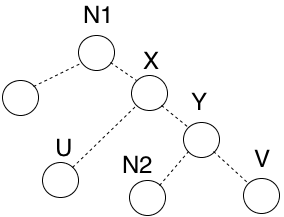
\includegraphics[width=60mm]{2b.png}
\caption{Ejemplo gráfico de la suposición}
\label{overflow}
\end{figure}  
  
  Entonces, sea l función de longitud entre dos nodos, l(U,V) = h(U) + h(V) - 2*h(X) y l(U,N2) = h(U) + h(N2) - 2*h(X), y como h(N2) $>$ h(U) por ser N2 el nodo más lejano o de mayor altura, esto implica que l(U,N2) $>$ l(U,V) y esto es absurdo por ser C1 el camino máximo.
  
  Por el absurdo, concluimos que U = N2, es decir, que N2 es un extremo del camino máximo.
\end{itemize}

Al obtener un extremo del camino máximo, otra ejecución de BFS desde el extremo encontrado caerá sobre el caso trivial de pertenecer al camino máximo y encontrará el camino más lejano a este, su otro extremo.

Teniendo los dos extremos, buscamos el camino máximo del árbol (secuencia de nodos) mediante la función Camino\_entre\_nodos. A continuación demostraremos que es correcta.

\begin{itemize}
\item Terminación:

La función recorre para cada nodo, de forma recursiva, sus nodos adyacentes, si o solo si, no han sido recorridos antes, por lo que el árbol se recorre una única vez por cada nodo, terminando al no tener nodos por recorrer.

\item  Resultado correcto:

Al recorrer una única vez cada nodo y como es un árbol (existe un camino para todo par de nodos), se recorrerá todo el árbol y eventualmente se llegará al nodo buscado. Al llegar al nodo buscado, la función devolverá true, haciendo que se agreguen los caminos recorridos hacia el hasta llegar al inicial.
\end{itemize}

Una vez obtenido el camino, el nodo que se encuentre en la mitad de este, será el nodo master, es decir, el nodo que se encuentra a menor distancia de todos los nodos.

Hay que probar que el nodo master seleccionado desde el camino máximo va a ser el master que queremos!
Supongamos ahora, que el nodo master no se encontrara en el camino máximo. (Falta)

Supongamos que el nodo master no se encontrara en la mitad del camino máximo, si no, en otra parte de este. Esto sería absurdo, ya que una elección diferente a la mitad, no cumpliría el estar a menor distancia posible de todos los nodos, ya que, estaría más cerca de alguno de sus extremos.

\paragraph{Verificación de correctitud}

\subsection{Preguntas adicionales}
Mostrar con un contraejemplo que es posible resolver las dos partes por separado de manera óptima pero que aún así haya una solución en la que la replicación termine en menos tiempo. Comentarposibles soluciones al problema.


¿Cómo se debe modificar la solución si en lugar de transmitir por broadcast se lo hace por
multicast ,es decir, se debe mandar un paquete a cada destino, sin hacer copias?


\subsection{Experimentos computacionales}


\subsubsection{Caso general}

\begin{figure}[H]
  \centering
  \dosgraficos{problema2-caso-general}
              {problema2-caso-general-n}
  \caption{Caso general}
\end{figure}


\subsubsection{Instancias aleatorias}

\begin{figure}[H]
  \centering
  \dosgraficos{problema2-instancias-aleatorias}
              {problema2-instancias-aleatorias-n}
  \caption{Instancias aleatorias}
\end{figure}



%%%%%%%%%%%%%%%%%%%%%%%%%%%%%%%%%%%%%%%%%%%%%%%%%%%%%%%%%%%%%%%%%%%%%%%%%%%%%%%
%% Problema 3: Transportes pesados                                           %%
%%%%%%%%%%%%%%%%%%%%%%%%%%%%%%%%%%%%%%%%%%%%%%%%%%%%%%%%%%%%%%%%%%%%%%%%%%%%%%%


\newpage

\section{Problema 3: Transportes pesados}

Una empresa que fabrica ladrillos tiene sus fábricas en varios puntos de una provincia. La misma se encarga de transportar los ladrillos a los clientes que están distribuísdos en distintas ciudades de la provincia.\\
Como las rutas de esta provincia no están preparadas para soportar el paso de los camiones, la empresa tiene que fortalecer las rutas para que puedan ser utilizadas por los camiones.\\
Dado que cada ruta tiene un costo de inversión proporcional a la longitud de la misma, se pide replanificar las rutas habituales de manera tal de minimizar los gastos que implicará el fortalecimiento de las rutas para que cada cliente pueda ser provisto desde al menos una fábrica.\\
La complejidad temporal del \textbf{peor caso} deberá ser \textbf{O($C^2$)} o bien \textbf{O(R$log$(C)).}

\textbf{Ejemplos del problema y sus soluciones:}

\textbf{Entrada}: 2 fábricas, 2 clientes y 4 rutas.
\begin{itemize}
\item{La lonitud de la ruta desde la fábrica 1 a la fábrica 2 es 1.}
\item{La lonitud de la ruta desde la fábrica 1 al cliente 1 es 4.}
\item{La lonitud de la ruta desde la fábrica 2 al cleinte 2 es 5.}
\item{La lonitud de la ruta desde el cliente 1 al cliente 2 es 7.}
\end{itemize}

\begin{figure}[H]
\centering
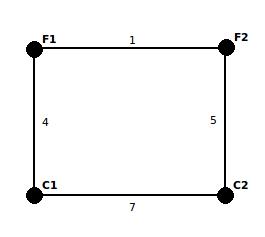
\includegraphics[width=60mm]{../ejemplo_graficos/CosoDosSubconjuntos.png}
\caption{Grafo inicial}
\label{1}
\end{figure} 

\begin{figure}[H]
\centering
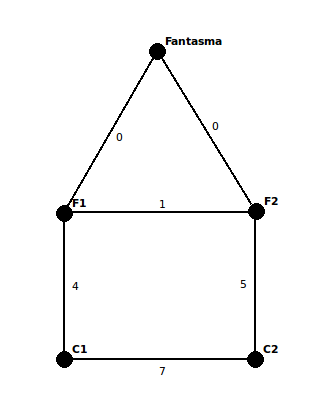
\includegraphics[width=60mm]{../ejemplo_graficos/CosoDosSubconjuntosConNodoFantasma.png}
\caption{Se le agrega el nodo \textit{fantasma}}
\label{2}
\end{figure} 

\begin{figure}[H]
\centering
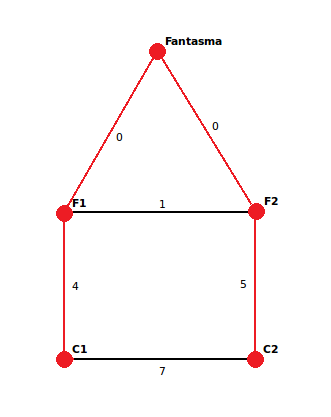
\includegraphics[width=60mm]{../ejemplo_graficos/CosoDosSubconjuntosConNodoFantasmaSolucion.png}
\caption{AGM con nodo \textit{fantasma}}
\label{3}
\end{figure} 

\begin{figure}[H]
\centering
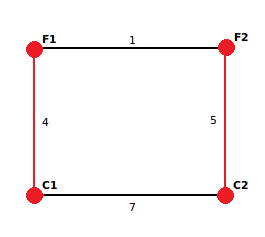
\includegraphics[width=60mm]{../ejemplo_graficos/CosoDosSubconjuntosSolucion.png}
\caption{Se le quita el nodo \textit{fantasma}}
\label{4}
\end{figure} 

\begin{figure}[H]
\centering
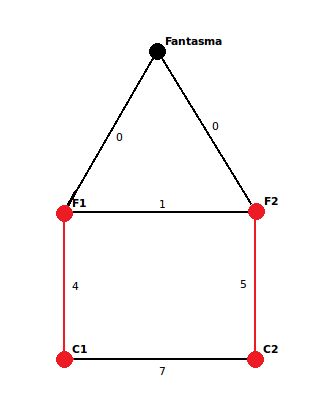
\includegraphics[width=60mm]{../ejemplo_graficos/CosoDosSubconjuntosSolucionSinFantasma.png}
\caption{Solución final}
\label{5}
\end{figure} 

\textbf{Salida}: Costo total de inversión 9. Las rutas utilizadas fueron:
\begin{itemize}
\item{de la fábrica 1 al cliente 1.}
\item{de la fábrica 2 al cliente 2.}
\end{itemize}

\subsection{Solución}

Dada una serie de aristas y sus respectivos costos, que representan las rutas entre clientes y fábricas y el costo de pavimentación, utilizamos para la resolución una modificación del conjuto de datos para luego aplicar el algoritmo de Kruskal con la estrucuta Disjoint-Set.

La idea de la utilización del algoritmo de Kruskal nace de la necesidad de conseguir un bosque de AGM's entre clientes y fábricas, lo que nos permitirá conseguir los caminos que los interconecten de mínimo costo. Como en nuestro caso, solo se necesita que una fábrica este conectada por una serie de rutas a otros clientes, creamos un nodo \textit{fantasma} al cuál le conectamos cada fábrica mediante una arista de costo cero para poder tener un único set que forzará a que el algoritmo solo conecte una única vez una fábrica con cada set disjunto.

El resultado obtenido será un árbol AGM al cual, al sacarle el nodo \textit{fantasma} y las aristas de las fábricas a este, como solo se unían los set disjuntos con una sola fábrica, se forma un bósque, donde los árboles de este tendran las rutas necesarias para pavimentar y minimizar el costo de inversión.

\subsubsection{Pseudocódigo}
\begin{pseudo}

\State ranking : vector de enteros

\State $tupla <nodo1 : entero, nodo2 : entero, costo : entero>$ es $ruta$
\Procedure{problema3}{nodos : entero, cantFabricas : entero, rutas : vector de ruta}
	\For{i=0 To Tamaño(parent)} parent[i] = i \EndFor						\Ode{C}
	\For{i=0 To Tamaño(ranking)} ranking[i] = 0 \EndFor						\Ode{C}

    \State camino\_minimo : vector de ruta									\Ode{1}
    \For{unsigned i = 0; i < cantFabricas; ++i}								\Ode{1}
        \State rutas.Agregar(ruta(i, nodos, 0))								\Ode{1}
    \EndFor

	

    \State Ordenar(rutas) ordenar de manera creciente las rutas por costo \Ode{R log R}

    \For{i = 0 To Tamaño(rutas)}
        \State set1 : entero = Find(nodo1(rutas[i]))						\Ode{1}
        \State set2 : entero = Find(nodo2(rutas[i]))						\Ode{1}
        \If{set1 != set2}													\Ode{1}
            \State Make\_union(set1, set2)									\Ode{1}
            \State camino\_minimo.Agregar(rutas[i])							\Ode{1}
        \EndIf    
    \EndFor

	 

    \State res : vector de rutas de tamaño (camino\_minimo.size() - cantFabricas)   \Ode{C}
    \For{i = cantFabricas To Tamaño(camino\_minimo)}
        \State res.Agregar(ruta(nodo1(camino\_minimo[i]), nodo2(camino\_minimo[i]), costo(camino\_minimo[i])))	\Ode{1}
    \EndFor
    \Return res
\EndProcedure

\end{pseudo}

\subsection{Complejidad}

Como se agrega un conjunto nuevo de aristas acotado por la cantidad de fábricas, se obtiene un costo de O(F) para crear las nuevas rutas que se conectarán al nodo \textit{fantasma}. Como R $>$ F, O(F) $\in$ O(R) acotando la cantidad de rutas a O(R).

Debido a que para el ordenamiento de las rutas, utilizamos la función Sort() de la STL de C++, se obtiene una costo de O(R * log R), siendo R rutas, lo que equivale a O(R * log $(C+F)^2$), siendo C clientes y F fábricas por ser C+F la mayor cantidad de aristas posibles. Por ser F menor que C, O(F) $\subset$ O(C), log($(C+F)^2$) $\subset$ log($C^2$). Siendo O($C^2$) la cota superior para la cantidad de aristas, la complejidad equivale a O(R * 2 log C) $\subset$ O(R * log C).

Como se utiliza el algoritmo de Kruskal, al igual que en el segundo problema, la complejidad de obtener los subconjuntos de rutas que unen clientes con fábricas es de O(R).

Como O(R) $\subset$ O(R * log C), la complejidad final del algoritmo es O(R * log C).
\subsection{Correctitud}
Un bosque con aristas de peso mínimo y una sola conexión a una fábrica para cada árbol, es una solución correcta, ya que, para todo árbol del bosque, sus nodos (clientes) y única fábrica (ya que más de una necesitaría otra ruta y no sería mínimo), estan conectados mediante las aristas de menor costo de pavimentación, haciendo que el costo sea mínimo.

Para demostrar la correctitud del algoritmo, debemos demostrar que Kruskal aplicado a la modificación realizada a nuestro conjunto de datos devuelve un AGM al que, al podarle el nodo \textit{fantasma} se convierte en un bosque de árboles, cada uno con clientes y una fábrica asociada conectados con costo mínimo.

Debido a que asumimos que los costos de pavimentación de todas las rutas son mayor a 0 (ya que el costo es proporcional a la longitud), en las primeras iteraciones (exactamente \#(F)) del algoritmo, se unirán todas las fábricas en único set. Por esta unión, Kruskal se encargará de unir una única vez una fábrica con los conjuntos de clientes. En las próximas iteraciones de Kruskal, el algoritmo se comportará  de la manera habitual.

Dada la solución obtenida por Kruskal, queremos ver que al podar el nodo fantasma y sus aristas, el bosque generado es mínimo.

Por el absurdo. Supongo que la solución obtenida no es óptima, esto implica que existe otro bosque solución el cuál tiene un costo menor. Para este bosque conecto sus fábricas con un nodo \textit{fantasma} y como los pesos de las aristas agregadas para conectar el nodo fantasma son 0, el árbol generado es AGM. Absurdo, ya que el árbol original devuelto por Kruskal ya era AGM.

Podemos concluir, por el absurdo que el bosque solución obtenido es el ópitmo en costo.


\subsection{Experimentos computacionales}


\newpage


\subsubsection{Peor caso}

\begin{figure}[H]
  \centering
  \tresgraficos{problema3-peor-caso}
               {problema3-peor-caso-logn}
               {problema3-peor-caso-n}
  \caption{Peor caso}
\end{figure}


\subsubsection{Mejor caso}

\begin{figure}[H]
  \centering
  \tresgraficos{problema3-mejor-caso}
               {problema3-mejor-caso-logn}
               {problema3-mejor-caso-n}
  \caption{Mejor caso}
\end{figure}


\subsubsection{Instancias aleatorias}

\begin{figure}[H]
  \centering
  \tresgraficos{problema3-instancias-aleatorias}
               {problema3-instancias-aleatorias-logn}
               {problema3-instancias-aleatorias-n}
  \caption{Instancias aleatorias}
\end{figure}


%%%%%%%%%%%%%%%%%%%%%%%%%%%%%%%%%%%%%%%%%%%%%%%%%%%%%%%%%%%%%%%%%%%%%%%%%%%%%%%
%% Conclusiones                                                              %%
%%%%%%%%%%%%%%%%%%%%%%%%%%%%%%%%%%%%%%%%%%%%%%%%%%%%%%%%%%%%%%%%%%%%%%%%%%%%%%%


\newpage

\section{Conclusiones}




%%%%%%%%%%%%%%%%%%%%%%%%%%%%%%%%%%%%%%%%%%%%%%%%%%%%%%%%%%%%%%%%%%%%%%%%%%%%%%%
%% Código fuente para el problema 1                                          %%
%%%%%%%%%%%%%%%%%%%%%%%%%%%%%%%%%%%%%%%%%%%%%%%%%%%%%%%%%%%%%%%%%%%%%%%%%%%%%%%


\newpage

\begin{appendices}

\section{Código fuente para el problema 1}


\subsection{problema1.h}

\subsection{problema1.cpp}




%%%%%%%%%%%%%%%%%%%%%%%%%%%%%%%%%%%%%%%%%%%%%%%%%%%%%%%%%%%%%%%%%%%%%%%%%%%%%%%
%% Código fuente para el problema 2                                          %%
%%%%%%%%%%%%%%%%%%%%%%%%%%%%%%%%%%%%%%%%%%%%%%%%%%%%%%%%%%%%%%%%%%%%%%%%%%%%%%%


\newpage

\section{Código fuente para el problema 2}


\subsection{problema2.h}

\subsection{problema2.cpp}



%%%%%%%%%%%%%%%%%%%%%%%%%%%%%%%%%%%%%%%%%%%%%%%%%%%%%%%%%%%%%%%%%%%%%%%%%%%%%%%
%% Código fuente para el problema 3                                          %%
%%%%%%%%%%%%%%%%%%%%%%%%%%%%%%%%%%%%%%%%%%%%%%%%%%%%%%%%%%%%%%%%%%%%%%%%%%%%%%%


\newpage

\section{Código fuente para el problema 3}


\subsection{problema3.h}

\subsection{problema3.cpp}


\end{appendices}

\end{document}